% =====================================================================
%  Ban rut gon -- chi trinh bay HAI SO DO kien truc
%
%  Bien dich:  xelatex SlideSoDo.tex   (chay 2 lan de co so trang)
%  Hinh ve:    ../figs/
%  Thoi luong: ~6 phut
%
%  GHI CHU NGUOI NOI nam trong cac khoi \note{...}
%  - Mac dinh: KHONG in ra.
%  - Muon xem: bo dau % o dong \setbeameroption ben duoi.
% =====================================================================
\documentclass[aspectratio=169,11pt]{beamer}

% \setbeameroption{show notes}
% \setbeameroption{show notes on second screen}

% ------------------------- Font & ngon ngu --------------------------
\usepackage{fontspec}
\setsansfont{texgyreheros}[
  Extension      = .otf,
  UprightFont    = *-regular,
  BoldFont       = *-bold,
  ItalicFont     = *-italic,
  BoldItalicFont = *-bolditalic ]
\usepackage[vietnamese]{babel}

% ------------------------------ Goi -------------------------------
\usepackage{graphicx}
\usepackage{booktabs}
\usepackage{tikz}
\usetikzlibrary{arrows.meta, positioning}
\usepackage{amsmath, amssymb}

% ----------------------------- Giao dien ----------------------------
\usetheme{default}
\usefonttheme{professionalfonts}
\setbeamertemplate{navigation symbols}{}

\definecolor{cPrimary}{HTML}{1F3A5C}
\definecolor{cAccent} {HTML}{C1440E}
\definecolor{cDet}    {HTML}{1B7F5C}
\definecolor{cMuted}  {HTML}{6B7280}
\definecolor{cBg}     {HTML}{F4F5F7}

\setbeamercolor{structure}{fg=cPrimary}
\setbeamercolor{frametitle}{fg=white, bg=cPrimary}
\setbeamercolor{title}{fg=cPrimary}
\setbeamercolor{alerted text}{fg=cAccent}
\setbeamercolor{block title}{fg=white, bg=cPrimary}
\setbeamercolor{block body}{bg=cBg}
\setbeamercolor{block title alerted}{fg=white, bg=cAccent}
\setbeamercolor{block body alerted}{bg=cBg}
\setbeamercolor{itemize item}{fg=cAccent}

\setbeamertemplate{itemize item}{\raisebox{0.15ex}{\tiny$\blacksquare$}}
\setbeamertemplate{blocks}[rounded][shadow=false]

\setbeamertemplate{frametitle}{%
  \nointerlineskip
  \begin{beamercolorbox}[wd=\paperwidth, ht=2.9ex, dp=1.3ex, leftskip=0.8em, rightskip=0.8em]{frametitle}
    \usebeamerfont{frametitle}\strut\insertframetitle\hfill
    {\footnotesize\color{white!75!cPrimary}\insertsectionhead}
  \end{beamercolorbox}
}
\setbeamerfont{frametitle}{size=\large, series=\bfseries}
\setbeamerfont{block title}{size=\normalsize, series=\bfseries}
\setbeamerfont{footline}{size=\tiny}

\setbeamertemplate{footline}{%
  \hbox{\begin{beamercolorbox}[wd=\paperwidth, ht=2.4ex, dp=1ex, leftskip=0.8em, rightskip=0.8em]{}
    \color{cMuted}\tiny Kiến trúc hệ thống AQG Toán\hfill\insertframenumber/\inserttotalframenumber
  \end{beamercolorbox}}
}
\setbeamerfont{note page}{size=\small}

% ----------------------------- Lenh tat ------------------------------
\newcommand{\dt}[1]{\textcolor{cDet}{\textbf{#1}}}
\newcommand{\punch}[1]{\begin{center}\alert{\large #1}\end{center}}
\newcommand{\capt}[1]{\vfill{\scriptsize\color{cMuted}#1\par}}

% ------------------------------ Tieu de ------------------------------
\title{\bfseries Kiến trúc hệ thống sinh câu hỏi trắc nghiệm Toán}
\subtitle{Hai sơ đồ}
\author{}
\date{}

\begin{document}

% =====================================================================
\begin{frame}[plain]
  \titlepage
  \vspace{-2em}
  \centering
  {\footnotesize\color{cMuted}Bản rút gọn --- chỉ trình bày hai sơ đồ kiến trúc}
\end{frame}

% =====================================================================
\section{Tổng thể}
\begin{frame}{Sơ đồ 1 --- Kiến trúc tổng thể}
  \vfill
  \begin{center}
    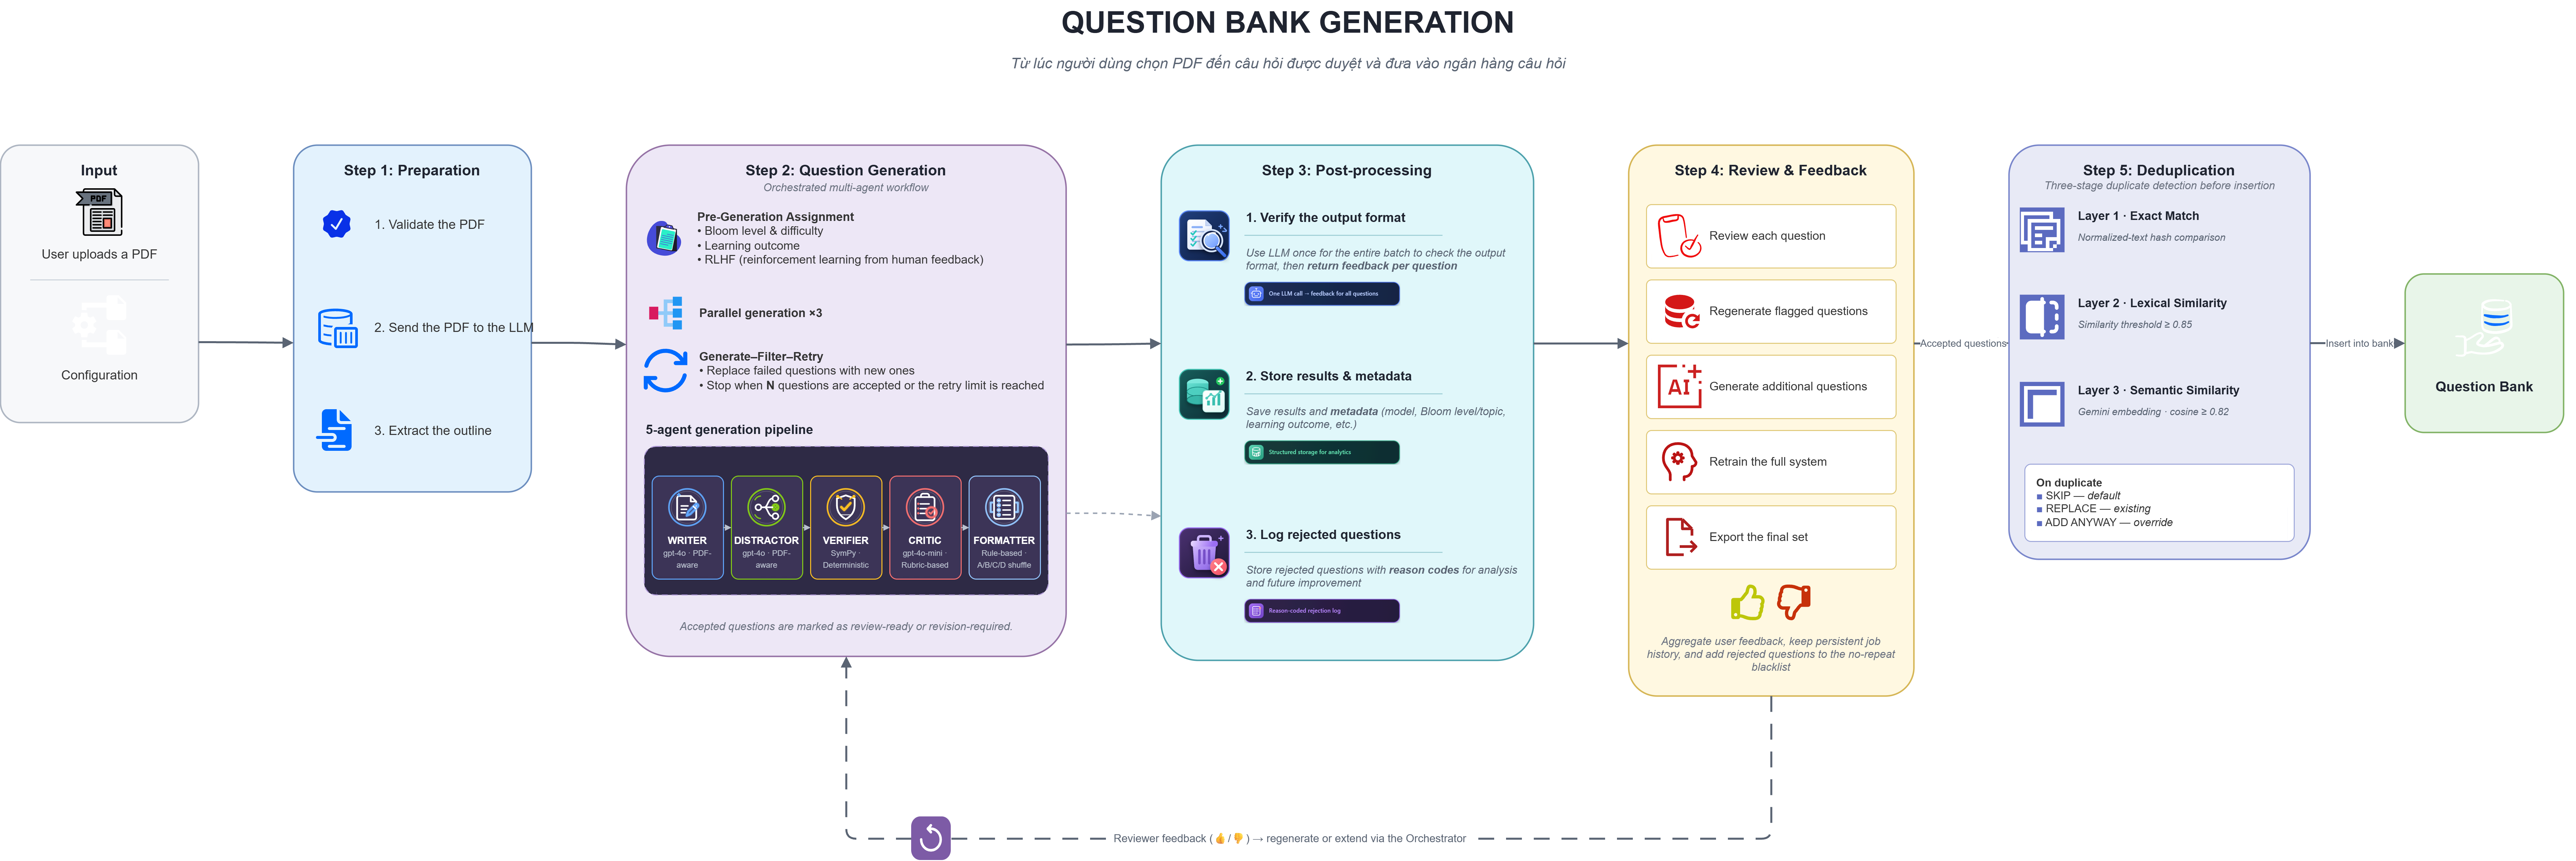
\includegraphics[width=\textwidth]{../figs/pipeline-tong-the.png}
  \end{center}
  \vfill
  \capt{Tài liệu đi qua năm giai đoạn từ trái sang phải. Chuỗi năm tác tử nằm bên trong giai đoạn \textcircled{\tiny 2}. Đường nét đứt phía dưới là vòng phản hồi người dùng.}
  \note{
    Đây là toàn cảnh hệ thống. Ba chỗ cần chỉ tay, theo đúng thứ tự:

    1. Dải màu đậm ở giữa --- chuỗi năm tác tử. Nó nằm BÊN TRONG giai đoạn sinh, và sẽ được phóng to ở sơ đồ thứ hai.

    2. Đường nét đứt phía dưới --- vòng phản hồi người dùng. Đánh giá ở khâu duyệt được đưa ngược về bộ điều phối để sinh lại hoặc sinh bổ sung, mà không cần tải lại tài liệu.

    3. Ba tầng khử trùng lặp ở cuối --- xếp theo chi phí tăng dần.

    Đừng đọc từng hộp. Để hội đồng nhìn tổng thể trước, chi tiết nói ở slide sau.
  }
\end{frame}

% =====================================================================
\begin{frame}{Đọc sơ đồ 1}
  \vfill
  \begin{columns}[T]
    \begin{column}{0.52\textwidth}
      \begin{block}{Năm giai đoạn}
        \small
        \begin{tabular}{@{}c l@{}}
          \textcircled{\scriptsize 1} & Chuẩn bị tài liệu \\[0.15em]
          \textcircled{\scriptsize 2} & Sinh câu hỏi --- \alert{đa tác tử, song song} \\[0.15em]
          \textcircled{\scriptsize 3} & Hậu xử lý \\[0.15em]
          \textcircled{\scriptsize 4} & Duyệt --- \alert{vòng lặp con người} \\[0.15em]
          \textcircled{\scriptsize 5} & Nhập ngân hàng \\
        \end{tabular}
      \end{block}
    \end{column}
    \begin{column}{0.48\textwidth}
      \begin{alertblock}{Ba chi tiết đáng chú ý}
        \small
        \begin{itemize}
          \item Chuỗi tác tử \textbf{nằm trong} giai đoạn \textcircled{\tiny 2}
          \item Nét đứt = phản hồi quay về bộ điều phối, \textbf{không tải lại tài liệu}
          \item Ba tầng khử trùng lặp xếp theo \textbf{chi phí tăng dần}
        \end{itemize}
      \end{alertblock}
    \end{column}
  \end{columns}
  \vfill
  \punch{Giai đoạn \textcircled{\small 1} chạy ngay khi \emph{chọn} tài liệu ---\\[0.2em] trước khi người dùng cấu hình xong.}
  \vfill
  \note{
    Bảng bên trái là năm giai đoạn theo đúng thứ tự trên sơ đồ.

    Khối bên phải là ba thứ dễ bỏ sót khi nhìn hình.

    Câu chốt dưới cùng: giai đoạn chuẩn bị được kích hoạt ngay khi người dùng chọn tài liệu --- tức là trước khi họ cấu hình xong. Đây thoạt nhìn là quyết định về trải nghiệm, nhưng có hệ quả kiến trúc: nó buộc phần đóng gói tài liệu phải tách rời hoàn toàn khỏi phần cấu hình sinh. Đổi lại, hệ thống dùng chính lượt đọc lướt đó để gợi ý ngược cấu hình cho người dùng.

    NẾU BỊ HỎI ba tầng khử trùng lặp là gì: trùng nguyên văn, gần trùng theo hình thái, và trùng ngữ nghĩa bằng vector nhúng. Tầng ba là tầng duy nhất bắt được cùng một bài toán diễn đạt khác đi hoặc thay số liệu.
  }
\end{frame}

% =====================================================================
\section{Chuỗi tác tử}
\begin{frame}{Sơ đồ 2 --- Chuỗi tác tử cho mỗi câu hỏi}
  \vfill
  \begin{center}
    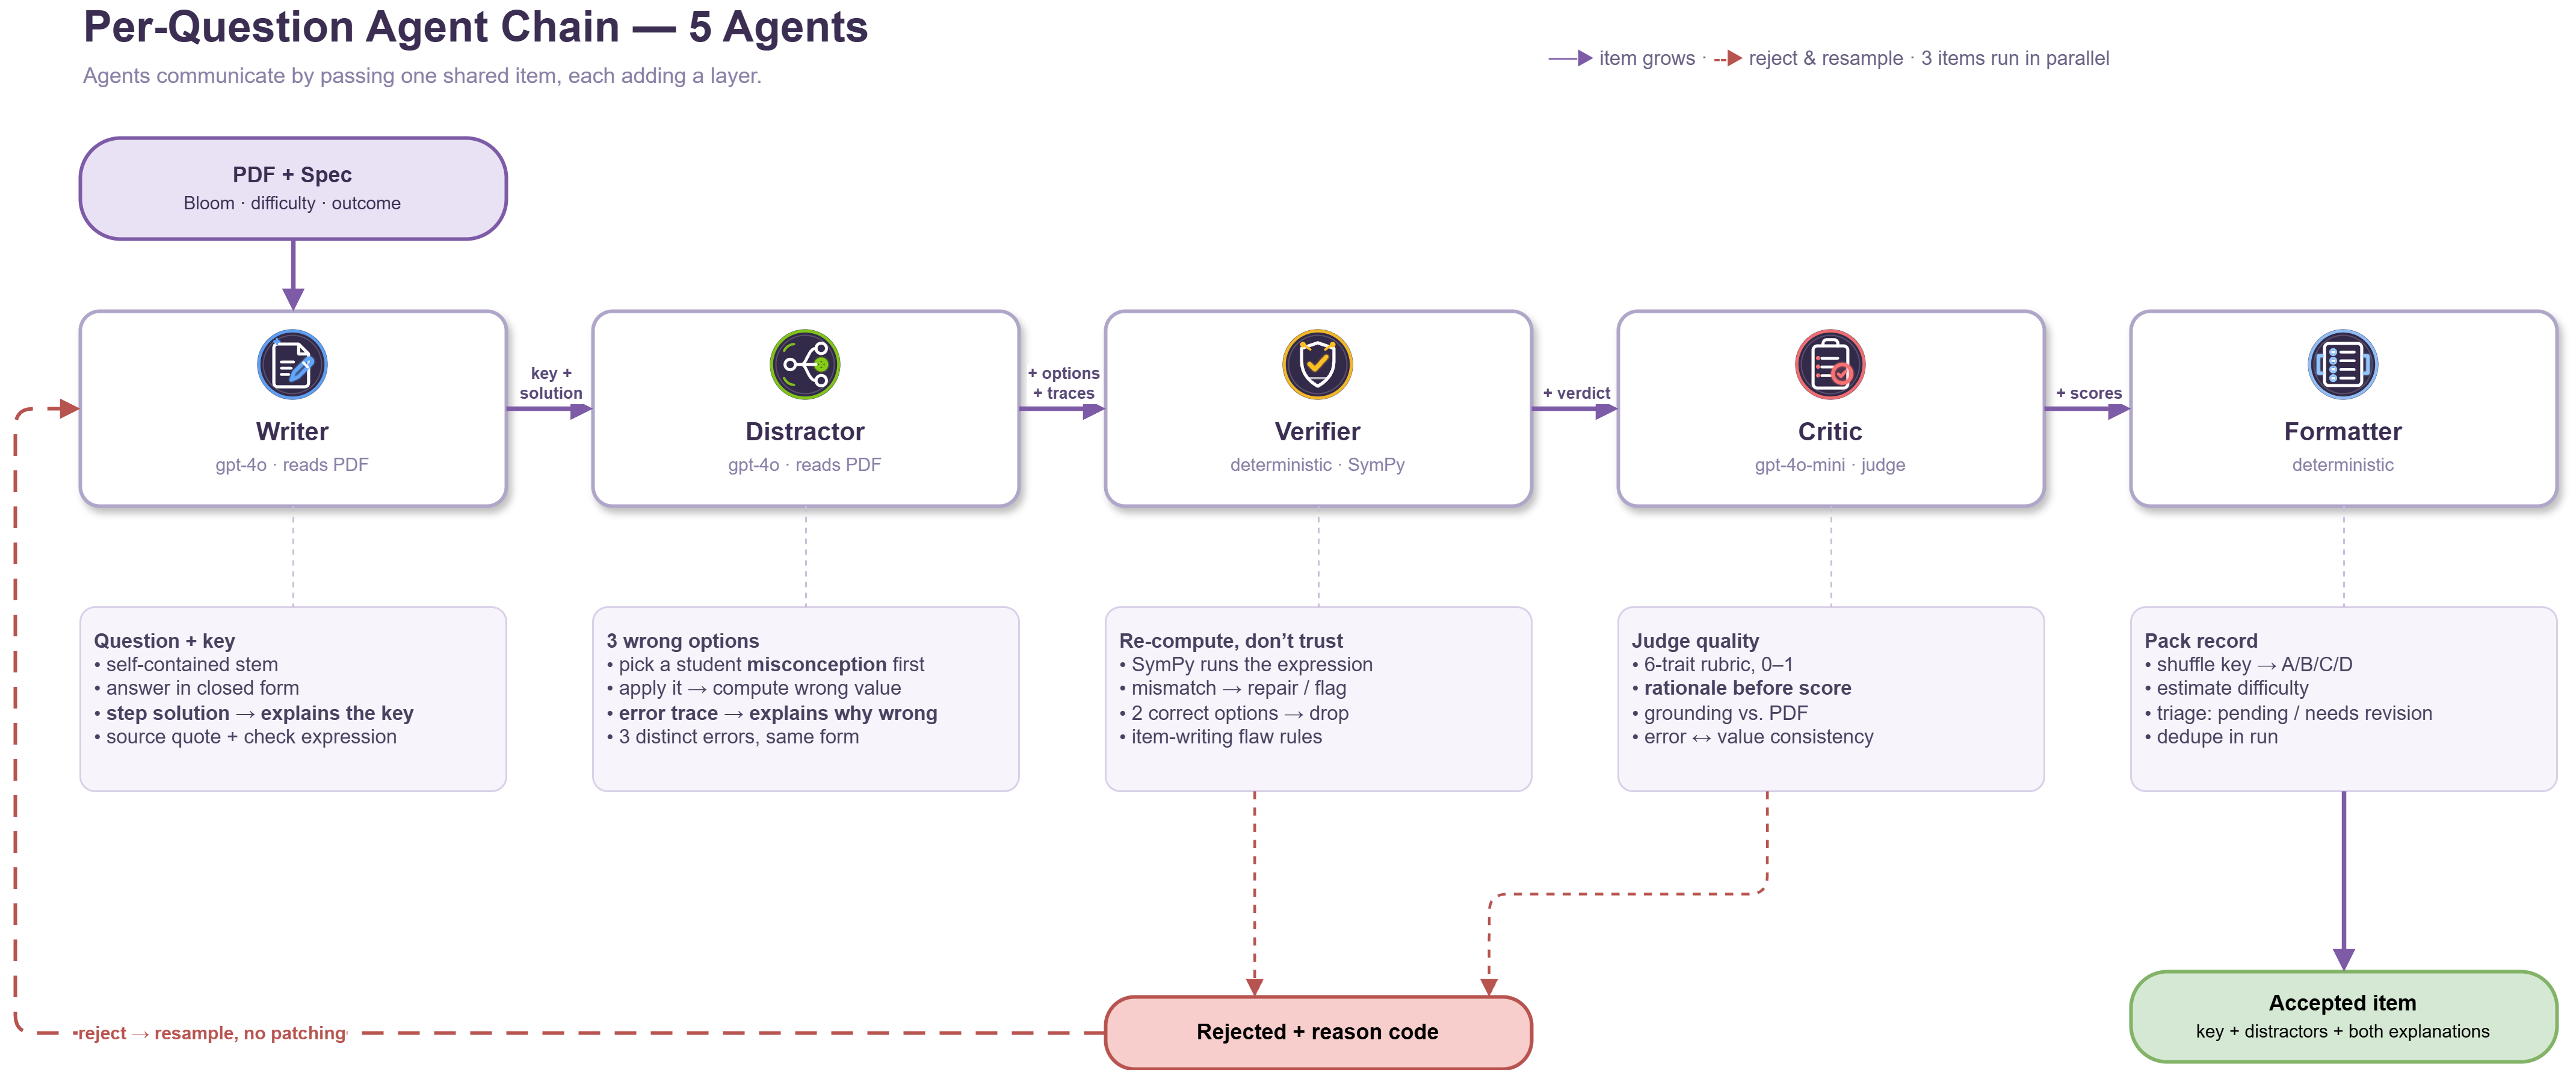
\includegraphics[width=\textwidth]{../figs/pipeline-5-agent.png}
  \end{center}
  \vfill
  \capt{Năm tác tử xử lý \emph{mỗi} câu hỏi. Nhãn trên mũi tên liền là dữ liệu mà tác tử đó bồi thêm vào bản ghi dùng chung. Đường nét đứt là các điểm loại bỏ.}
  \note{
    Đây là phóng to của giai đoạn 2 ở sơ đồ trước. Chuỗi này chạy cho MỖI câu hỏi.

    Ba điểm cần nói:

    1. Các tác tử giao tiếp một chiều --- chúng truyền nhau một bản ghi dùng chung, mỗi tác tử bồi thêm một lớp dữ liệu. Đó là các nhãn trên mũi tên liền.

    2. Hai hộp có màu khác là hai tác tử thuần tính toán --- Verifier và Formatter. Chúng không gọi mô hình ngôn ngữ nào cả.

    3. Các đường nét đứt là điểm loại bỏ. Mọi câu bị loại đều được ghi kèm mã lý do, và dẫn tới sinh lại một câu mới --- không vá câu cũ.
  }
\end{frame}

% =====================================================================
\begin{frame}{Đọc sơ đồ 2}
  \vspace{0.4em}
  \begin{center}
    \small
    \begin{tabular}{@{}c l l@{}}
      \toprule
      \# & \textbf{Tác tử} & \textbf{Nhiệm vụ} \\
      \midrule
      1 & Writer         & Đề, đáp án, lời giải, trích dẫn, biểu thức kiểm chứng \\
      2 & Distractor     & Ba phương án nhiễu \\
      3 & \dt{Verifier}  & \dt{Thuần tính toán} --- kiểm chứng toán học \\
      4 & Critic         & Chấm bám nguồn và sáu tiêu chí rubric \\
      5 & \dt{Formatter} & \dt{Thuần tính toán} --- đóng gói, trộn phương án, phân luồng \\
      \bottomrule
    \end{tabular}
  \end{center}
  \vfill
  \begin{columns}[T]
    \begin{column}{0.5\textwidth}
      \begin{block}{Mũi tên liền}
        Bản ghi dùng chung, mỗi tác tử \textbf{bồi thêm một lớp dữ liệu}.
      \end{block}
    \end{column}
    \begin{column}{0.5\textwidth}
      \begin{alertblock}{Mũi tên nét đứt}
        Điểm loại bỏ $\Rightarrow$ \textbf{sinh lại một câu mới}, không vá câu cũ. Mọi lần loại đều ghi kèm mã lý do.
      \end{alertblock}
    \end{column}
  \end{columns}
  \vfill
  \punch{\dt{Hai trong năm} tác tử chạy bằng chương trình ---\\[0.2em] chúng không gọi mô hình ngôn ngữ nào cả.}
  \vfill
  \note{
    Bảng liệt kê năm tác tử theo đúng thứ tự trên sơ đồ.

    Hai dòng màu xanh là hai tác tử thuần tính toán. Ba tác tử còn lại dùng mô hình ngôn ngữ, và cả ba đều đọc trực tiếp tài liệu PDF.

    Câu chốt là điểm quan trọng nhất của cả hai sơ đồ: tỉ lệ hai trên năm tác tử thuần tính toán. Nguyên tắc đằng sau là "việc gì máy tính được chính xác thì không giao cho mô hình ngôn ngữ".

    NẾU BỊ HỎI vì sao không có tác tử sửa lỗi: đây là lựa chọn có chủ ý. Một câu đã sửa mang theo lịch sử của phiên bản hỏng, và các ràng buộc chéo giữa đáp án, lời giải, biểu thức kiểm chứng và mô tả lỗi rất dễ bất nhất sau khi vá cục bộ.
  }
\end{frame}

% =====================================================================
\begin{frame}{Hai sơ đồ nối với nhau thế nào}
  \vspace{0.8em}
  \begin{center}
  \begin{tikzpicture}[
      stage/.style = {draw=cPrimary, fill=cBg, rounded corners=3pt, minimum height=2.6em, text width=2.1cm, align=center, font=\small},
      big/.style   = {draw=cAccent, fill=cAccent!10, line width=1pt, rounded corners=3pt, minimum height=2.6em, text width=2.1cm, align=center, font=\small\bfseries},
      ar/.style    = {-{Latex[length=1.8mm]}, draw=cPrimary!70, thick} ]
    \node[stage]                     (s1) {\textcircled{\tiny 1}\\Chuẩn bị};
    \node[big,   right=0.45cm of s1] (s2) {\textcircled{\tiny 2}\\Sinh câu hỏi};
    \node[stage, right=0.45cm of s2] (s3) {\textcircled{\tiny 3}\\Hậu xử lý};
    \node[stage, right=0.45cm of s3] (s4) {\textcircled{\tiny 4}\\Duyệt};
    \node[stage, right=0.45cm of s4] (s5) {\textcircled{\tiny 5}\\Ngân hàng};
    \draw[ar] (s1) -- (s2); \draw[ar] (s2) -- (s3);
    \draw[ar] (s3) -- (s4); \draw[ar] (s4) -- (s5);

    \node[below=1.5cm of s2, font=\small, text=cAccent, align=center] (z)
      {\textbf{Sơ đồ 2} phóng to giai đoạn này\\{\footnotesize chạy một lần cho \emph{mỗi} câu hỏi}};
    \draw[-{Latex[length=1.8mm]}, draw=cAccent, dashed, thick] (z) -- (s2);
  \end{tikzpicture}
  \end{center}
  \vfill
  \punch{Sơ đồ 1 là \emph{đường đi của tài liệu}.\\[0.2em] Sơ đồ 2 là \emph{đường đi của một câu hỏi}.}
  \vfill
  \note{
    Slide chốt. Điểm cần làm rõ để hội đồng không nhầm hai sơ đồ:

    Sơ đồ 1 mô tả đường đi của TÀI LIỆU --- chạy một lần cho cả lượt sinh.

    Sơ đồ 2 mô tả đường đi của MỘT CÂU HỎI --- chạy lặp lại, mỗi câu một lần, và các câu chạy song song với nhau theo từng đợt.

    Nói cách khác, sơ đồ 2 nằm gọn bên trong ô số 2 của sơ đồ 1.
  }
\end{frame}

% =====================================================================
\begin{frame}[plain]
  \vfill
  \centering
  {\Huge\bfseries\color{cPrimary} Cảm ơn}\\[1em]
  {\large\color{cMuted} Câu hỏi và thảo luận}
  \vfill
\end{frame}

\end{document}
